\newpage
\pagebreak

\section{Training Details}
\label{app:compute}
All implementations were done with PyTorch~\citep{paszke2019pytorch} and Huggingface Transformers~\citep{wolf-etal-2020-transformers}. All model training runs are done on NVIDIA A6000 and A100 GPUs and last \num{96} hours at maximum.

\section{Effect of Model Scale}
\label{app:scaling}
We run the experiments on composition with larger model scales with $|\mathcal{E}|=2000$ and $\phi \in \{5.4, 9.0, 18.0\}$. The results are shown in Figure~\ref{fig:scale}. Overall, it could be seen that scaling up the model won't qualitatively change the model's generalization behaviors, and the main pattern is that larger models converge in fewer optimization steps, which shares with prior findings~\citep{tirumala2022memorization, pmlr-v119-li20m}.

\begin{figure}[h]
\centering
\begin{subfigure}{0.48\textwidth}
    \centering
    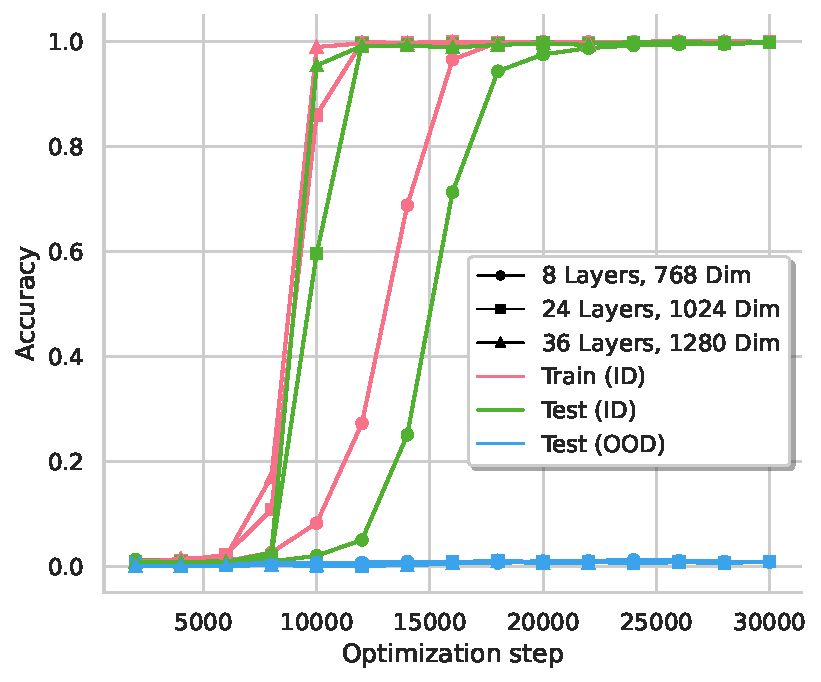
\includegraphics[width=\textwidth]{fig/scale180.pdf}
    \caption{$\phi=18.0$.}
\end{subfigure}
\begin{subfigure}{0.48\textwidth}
    \centering
    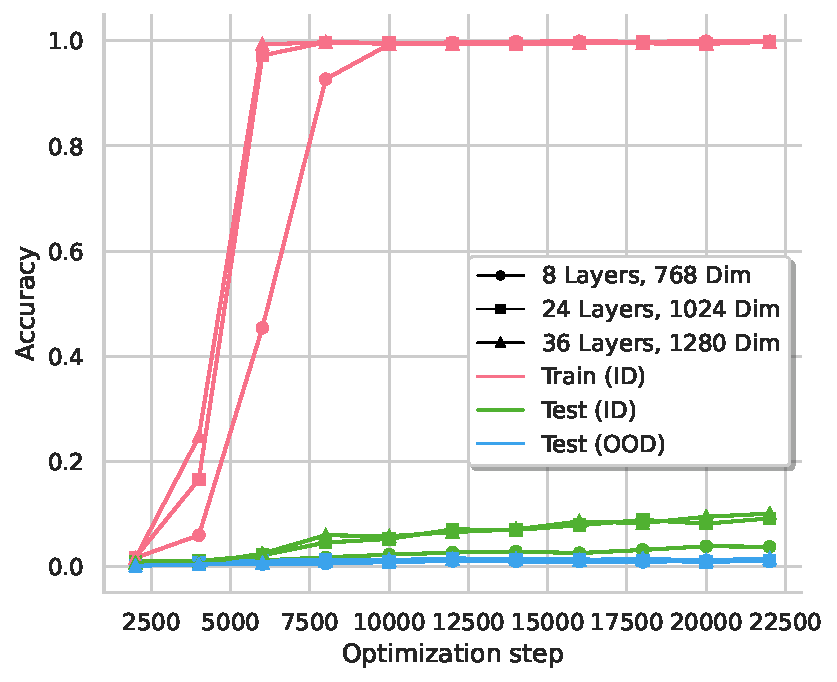
\includegraphics[width=\textwidth]{fig/scale54.pdf}
    \caption{$\phi=5.4$.}
\end{subfigure}
\begin{subfigure}{0.70\textwidth}
    \centering
    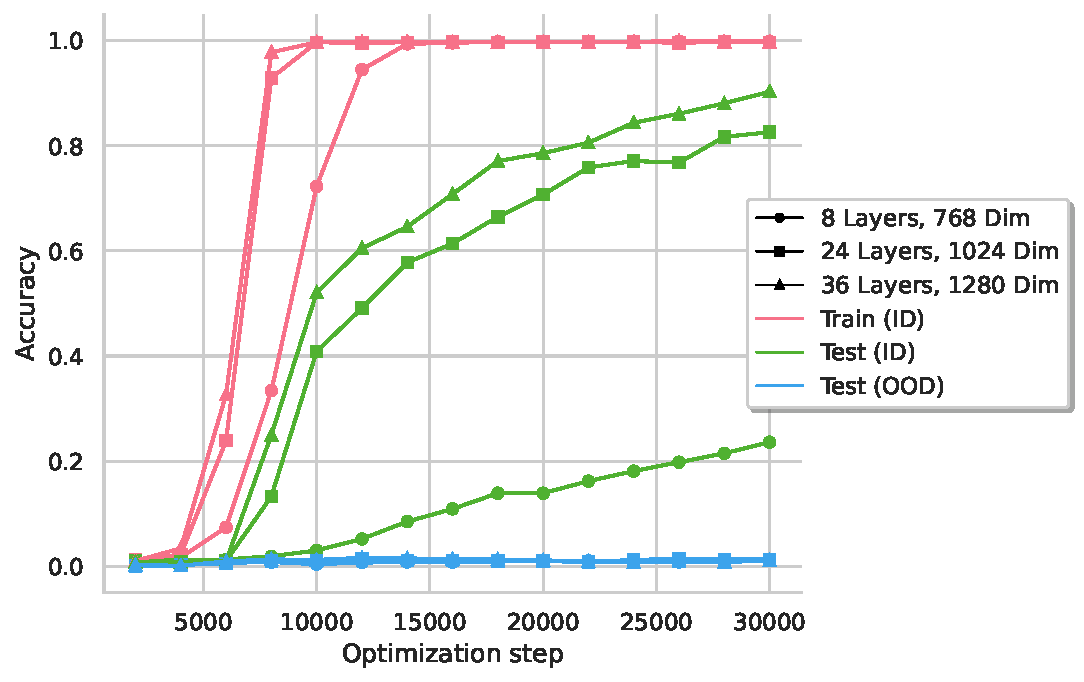
\includegraphics[width=\textwidth]{fig/scale90.pdf}
    \caption{$\phi=9.0$.}
\end{subfigure}
\caption{Results for different model scales across different $\phi$. Larger models converge in fewer optimization steps, but have no qualitative changes on the learned behaviors.}
\label{fig:scale}
\end{figure}

\section{Effect of Tokenizations}
\label{app:tokenization}
In the experiments in our main content, tokenization is done by having a unique token for each entity.\footnote{Preliminary experiments show that tokenization of the relations does not exhibit notable impacts, which is expected since relations are always explicitly given.} This is different from how real-world entities are typically tokenized---in practice, entities are usually multi-token, and different entities could share tokens at different positions. We investigate the effect of tokenizations on the composition task by having two tokens for each entity (resembling the first name and last name of a person) in the setting with $|\mathcal{E}|=2000$ and $\phi=12.6$. We generate a set of unique first names and a set of unique last names with equal size from which the two tokens for each entity are randomly chosen (we make sure each entity gets a unique ordered pair of tokens). We define \textit{token multiplicity} to be the number of entities that share the same first/last name. For example, when the size of the set of first/last names is \num{50}, the token multiplicity would be $2000/50=40$.

Figure~\ref{fig:tokenization}(a) shows the ID test results, where the training and OOD results are the same from earlier (training performance saturates quickly, OOD result remains zero). It can be seen that a larger token multiplicity would delay the generalization, which is expected to a certain degree since the scale of the model is effectively smaller due to having fewer tokens in the vocabulary. Nevertheless, ID generalization always happens. We also run linear probing on $S[5,r_1]$ throughout training to predict the second token of the bridge entity $b$ in the setting with token multiplicity \num{40},\footnote{Recall that $S[5,r_1]$ is the state that encodes the bridge entity in the generalizing circuit (Figure~\ref{fig:circuit_composition}(a))}, where the results are shown in Figure~\ref{fig:tokenization}(b). It can be seen that the second token of $b$ can be perfectly decoded from $S[5,r_1]$ after grokking, and the decodability improves throughout grokking. This suggests that for the multi-token case, the model is additionally storing the second token of $b$ into $S[5,r_1]$ throughout grokking, which may be another factor that further delays the speed of grokking. These results also share with recent findings that in many cases, tokens beyond the immediate next token are linearly encoded in the hidden states~\citep{wu2024language, pal-etal-2023-future, belrose2023eliciting, cai2024medusa}.

In summary, different tokenizations affect the results in rather expected ways, and do not influence our main findings and conclusions.

\begin{figure}[h]
\centering
\begin{subfigure}{0.48\textwidth}
    \centering
    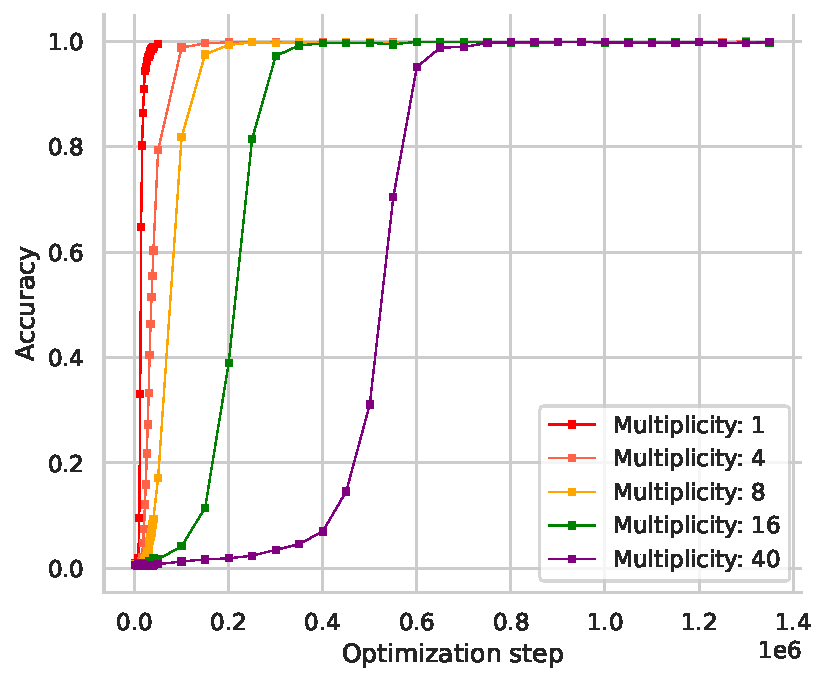
\includegraphics[width=\textwidth]{fig/token_mult.pdf}
    \caption{}
\end{subfigure}
\begin{subfigure}{0.48\textwidth}
    \centering
    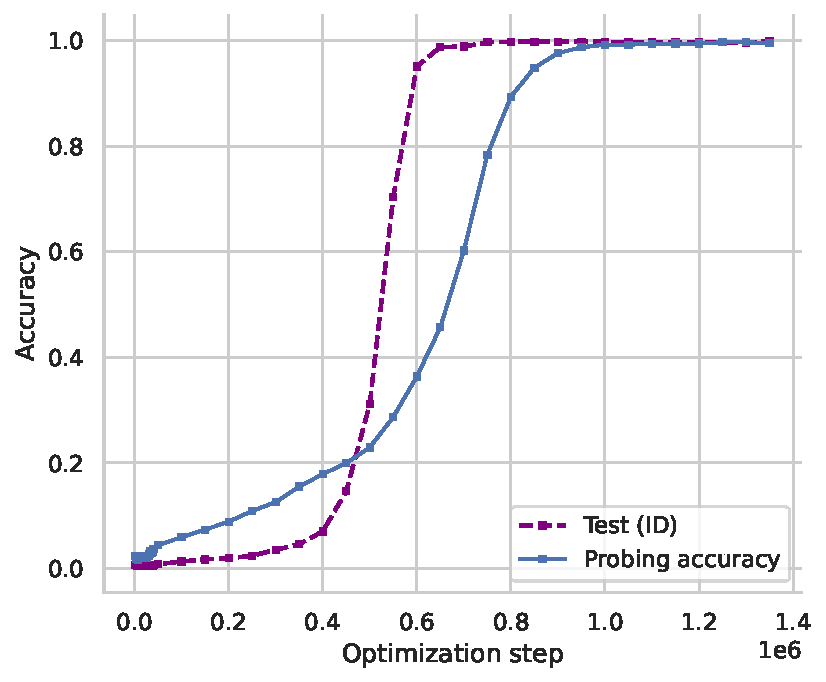
\includegraphics[width=\textwidth]{fig/probing.pdf}
    \caption{}
\end{subfigure}
\caption{(a) ID generalization across different token multiplicity. (b) Probing accuracy on the second token of $b$ at $S[5, r_1]$.}
\label{fig:tokenization}
\end{figure}

\section{More Details on Circuit Analysis}
\label{app:circuit}
\subsection{Composition}
We run causal tracing on hidden states in layer \num{1}-\num{7} and every position, where the target is the final prediction state $S[8,r_2]$. The changes in the strengths are monotone and smooth, and we show in Figure~\ref{fig:circuit_composition_full} the strengths for the model checkpoint at the start and end of grokking, and also their difference (same as Figure~\ref{fig:circuit_composition}(b)). We also find that after grokking, the state $S[5,r_2]$ (which encodes $r_2$) is not affected by perturbing the input $h$ or $r_1$. 

\noindent\textbf{Deriving the generalizing circuit}. Starting from the \num{9} states in layers $0,5,8$ we can directly eliminate $S[8,h]$ and $S[8,r_1]$ since they have no computational paths connecting to $S[8,r_2]$. $S[5,h]$ can be eliminated as could be seen by Figure~\ref{fig:circuit_composition_full}(c). The connections from $S[0,h]$ and $S[0,r_1]$ to $S[5,r_2]$ could be eliminated as mentioned earlier.

\begin{figure}[h]
\centering
\begin{subfigure}{0.30\textwidth}
    \centering
    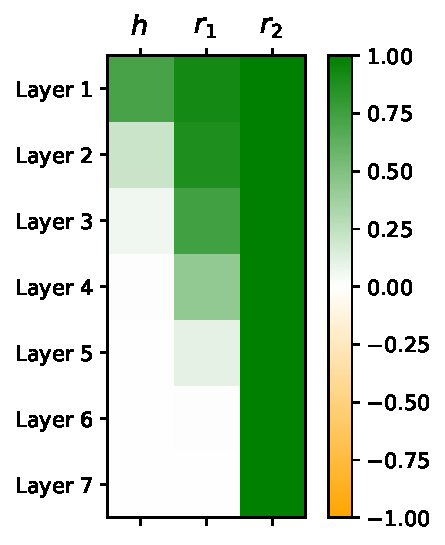
\includegraphics[width=\textwidth]{fig/causal_composition_before.pdf}
    \caption{}
\end{subfigure}
\begin{subfigure}{0.30\textwidth}
    \centering
    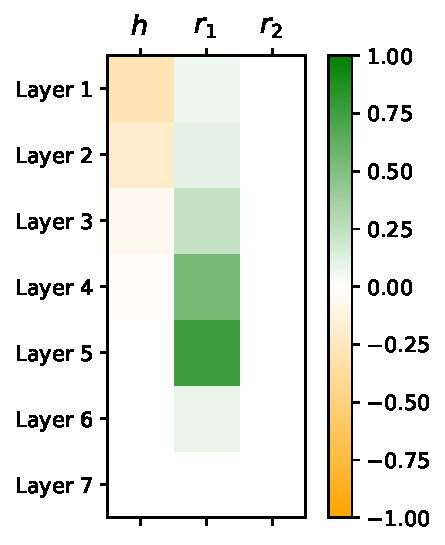
\includegraphics[width=\textwidth]{fig/causal_composition_diff.pdf}
    \caption{}
\end{subfigure}
\begin{subfigure}{0.30\textwidth}
    \centering
    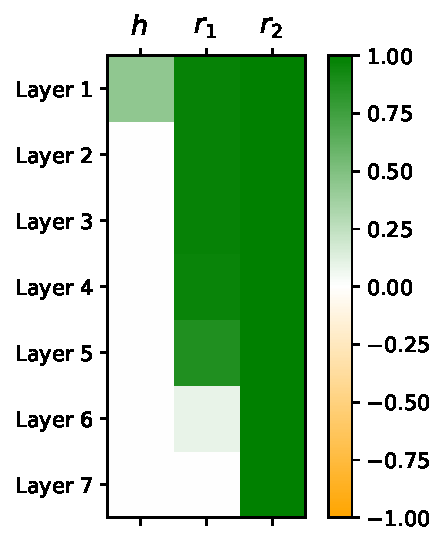
\includegraphics[width=\textwidth]{fig/causal_composition_after.pdf}
    \caption{}
\end{subfigure}
\caption{Causal strengths on composition task, with the final prediction $S[8,r_2]$ as the target. (a) Start of grokking. (b) Change during grokking. (c) End of grokking.}
\label{fig:circuit_composition_full}
\end{figure}

\subsection{Comparison}
Figure~\ref{fig:circuit_comparison_full} includes the causal tracing results where the target is the prediction state $S[8,e_2]$, and Figure~\ref{fig:circuit_comparison_v2_full} includes the results with the target state $S[5,e_2]$. It can be seen that after grokking, $S[5,e_2]$ does not depend on $e_1$, which gives the generalization circuit in Figure~\ref{fig:circuit_comparison}(a).

Figure~\ref{fig:label_space} shows the rank (via logit lens) of the three relations $\{a_<,a_=,a_>\}$ in the label space at state $S[7,a]$, where we use Recall@3 as the measure. It can be seen that $S[7,a]$ encodes the label space throughout grokking. 

\begin{figure}[h]
\centering
\begin{subfigure}{0.30\textwidth}
    \centering
    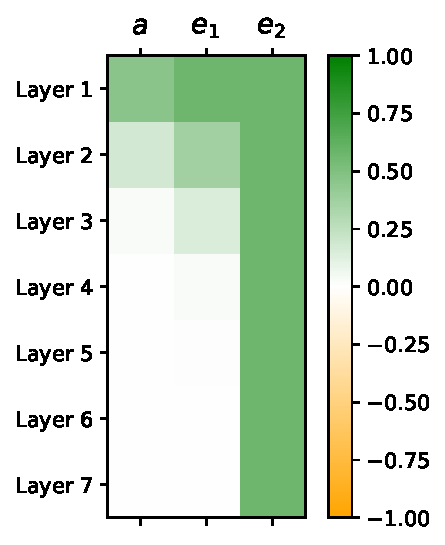
\includegraphics[width=\textwidth]{fig/causal_comparison_before.pdf}
    \caption{}
\end{subfigure}
\begin{subfigure}{0.30\textwidth}
    \centering
    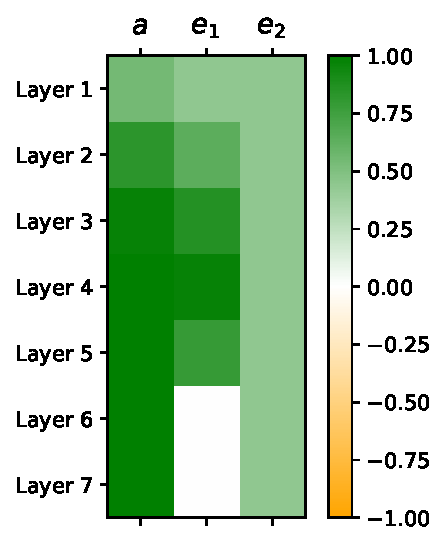
\includegraphics[width=\textwidth]{fig/causal_comparison_diff.pdf}
    \caption{}
\end{subfigure}
\begin{subfigure}{0.30\textwidth}
    \centering
    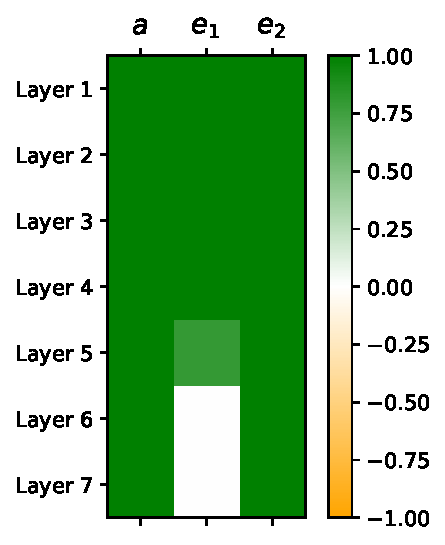
\includegraphics[width=\textwidth]{fig/causal_comparison_after.pdf}
    \caption{}
\end{subfigure}
\caption{Causal strengths on comparison task, with the final prediction $S[8, e_2]$ as the target. (a) Start of grokking. (b) Change during grokking. (c) End of grokking.}
\label{fig:circuit_comparison_full}
\end{figure}

\begin{figure}[h]
\centering
\begin{subfigure}{0.30\textwidth}
    \centering
    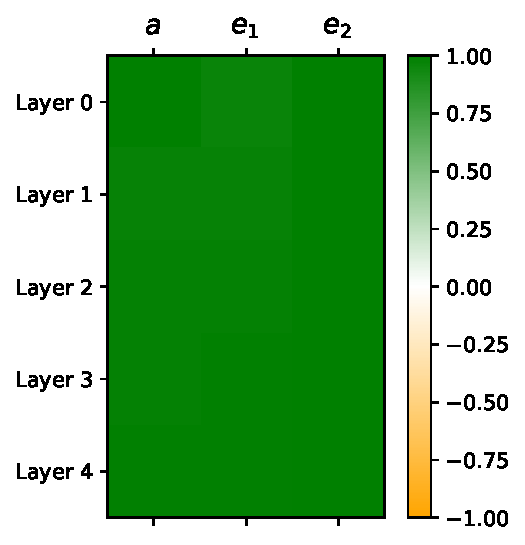
\includegraphics[width=\textwidth]{fig/causal_comparison_v2_before.pdf}
    \caption{}
\end{subfigure}
\begin{subfigure}{0.30\textwidth}
    \centering
    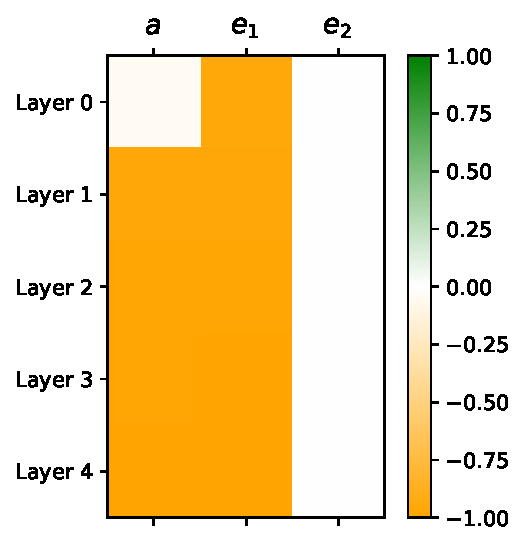
\includegraphics[width=\textwidth]{fig/causal_comparison_v2_diff.pdf}
    \caption{}
\end{subfigure}
\begin{subfigure}{0.30\textwidth}
    \centering
    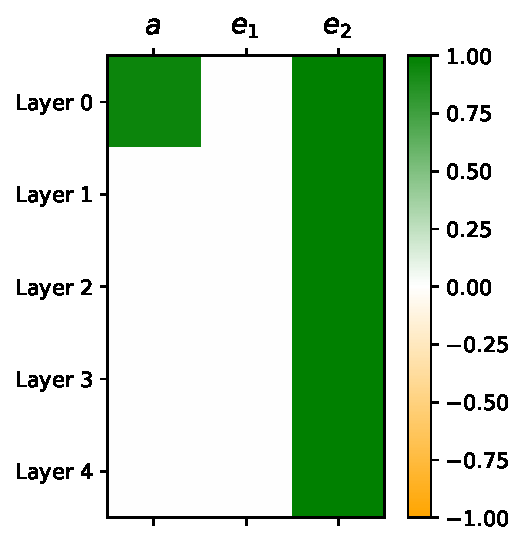
\includegraphics[width=\textwidth]{fig/causal_comparison_v2_after.pdf}
    \caption{}
\end{subfigure}
\caption{Causal strengths on comparison task, with $S[5, e_2]$ as the target. (a) Start of grokking. (b) Change during grokking. (c) End of grokking.}
\label{fig:circuit_comparison_v2_full}
\end{figure}

\begin{figure}[h]
\centering
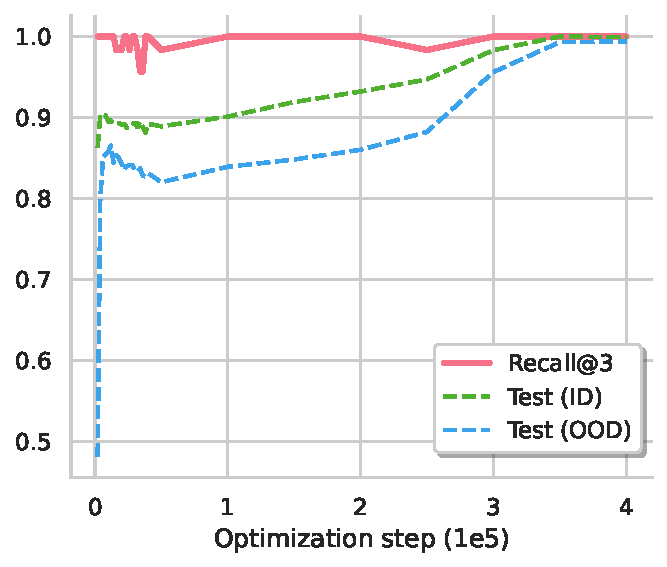
\includegraphics[width=0.6\textwidth]{fig/label_space.pdf}
\caption{For the comparison task, $S[7,a]$ encodes the label space throughout grokking.}
\label{fig:label_space}
\end{figure}


\section{Additional Results}
\label{app:other_results}

\subsection{Weight decay}
\label{app:wd}
Figure~\ref{fig:wd} shows the ID generalization performance when varying the degree of weight decay ($|\mathcal{E}|=2000$ and $\phi=9.0$). It can be seen that a larger weight decay can improve the speed of grokking, and vice versa.

\begin{figure}[h]
\centering
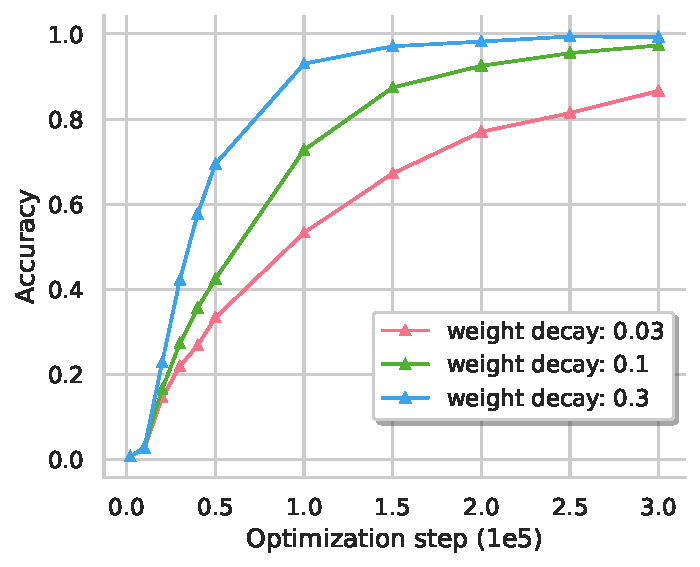
\includegraphics[width=0.6\textwidth]{fig/wd.pdf}
\caption{Effect of weight decay. A larger weight decay can improve the speed of grokking, and vice versa.}
\label{fig:wd}
\end{figure}

\subsection{Transformer with parameter sharing}
\label{app:ut}

We share the parameters of the first \num{4} layers and the last \num{4} layers, similar as in Universal Transformer~\citep{dehghani2018universal}. This would allow the model to share the knowledge in the upper and lower layers. The results on the setting with $|\mathcal{E}|=2000$ and $\phi=12.6$ are shown in Figure~\ref{fig:ut}. It could be seen that the parameter-sharing scheme can unlock OOD generalization, even though it is gained much more slowly than ID generalization during grokking.

\begin{figure}[h]
\centering
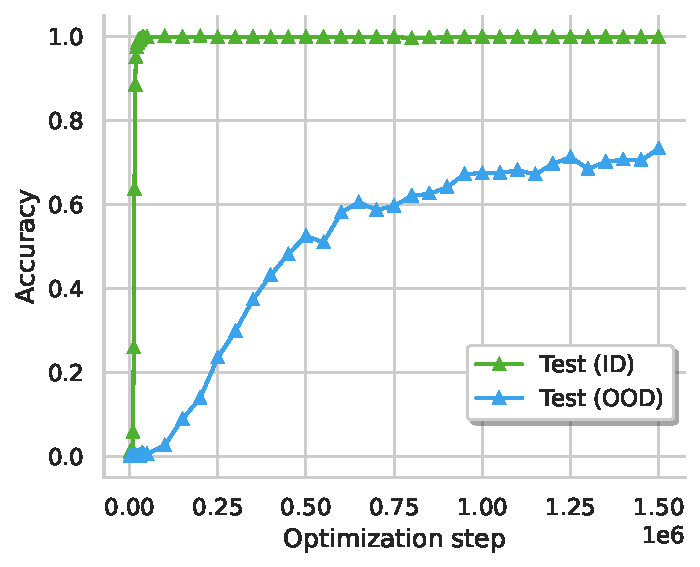
\includegraphics[width=0.6\textwidth]{fig/OOD.pdf}
\caption{OOD accuracy of the shared-parameter transformer model.}
\label{fig:ut}
\end{figure}

\subsection{Comparison task across different inferred/atomic ratio}
\label{app:comparison_phi}
Figure~\ref{fig:comp_phi} includes the result for $\phi \in \{3.6, 7.2, 9.0, 12.6\}$ for the comparison task. It can be seen that a higher ratio $\phi$ would give a higher generalization speed, consistent with the results in the composition task.

\begin{figure}[h]
\centering
\begin{subfigure}{0.48\textwidth}
    \centering
    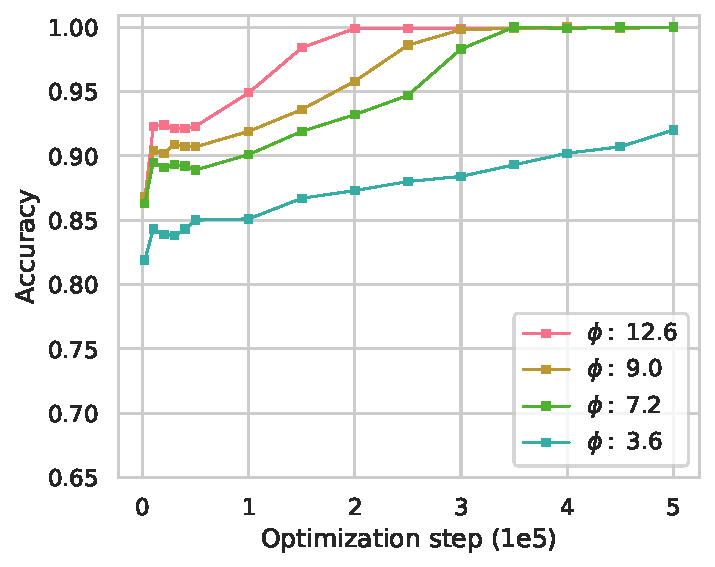
\includegraphics[width=\textwidth]{fig/comparison_ID.pdf}
    \caption{ID accuracy.}
\end{subfigure}
\begin{subfigure}{0.48\textwidth}
    \centering
    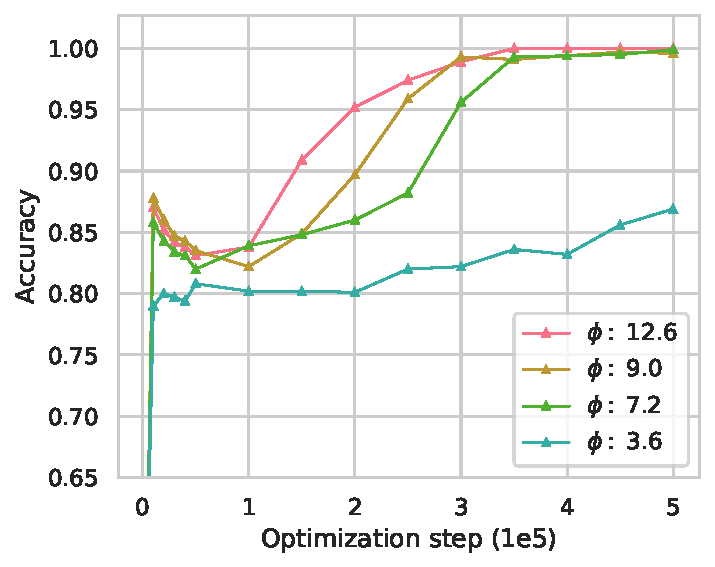
\includegraphics[width=\textwidth]{fig/comparison_OOD.pdf}
    \caption{OOD accuracy.}
\end{subfigure}
\caption{Results for the comparison task across different ratio $\phi$.}
\label{fig:comp_phi}
\end{figure}

\section{Complex Reasoning Task}
\label{app:hard_reasoning}

For the complex reasoning task, for each attribute, we include \num{3}\% random facts from the comparisons between ID and OOD entities and the comparisons between ID and ID entities. In total, the training set contains \num{18}K ID atomic facts, \num{437}K (ID, ID) comparisons, and \num{108}K (ID, OOD) comparisons, altogether \num{563}K facts (\num{28}K on average for each attribute). For translating the facts into natural language for testing LLMs with non-parametric memory, we always use the attribute \textit{age}\footnote{Recall that we test each attribute separately by grouping the facts/queries.} (we find that the choice of attribute does not exhibit notable impact) and the templates ``The age of \{entity\} is \{attribute value\}.'' and ``\{entity \num{1}\} is \{younger than/older than/in the same age as\} \{entity \num{2}\}.'' for atomic facts and comparisons. The entities are mapped to distinct random names generated by a random generator.\footnote{https://pypi.org/project/names/} We also try different mappings (e.g., unique IDs) and templates, and find the results to be consistent. All (retrieved) facts are randomly permuted and concatenated before being loaded into the LLM context.

The train/test accuracy, and also the accuracy of inferring the attribute values of the query entities (which we test using the same format as the atomic facts in training) are included in Figure~\ref{fig:hr}. It could be seen that, during grokking, the model gradually locates the ground truth attribute values of the query entities (note that the model is not explicitly encouraged or trained to do this), allowing the model to solve the problem efficiently with near-perfect accuracy. 

\begin{figure}[h]
\centering
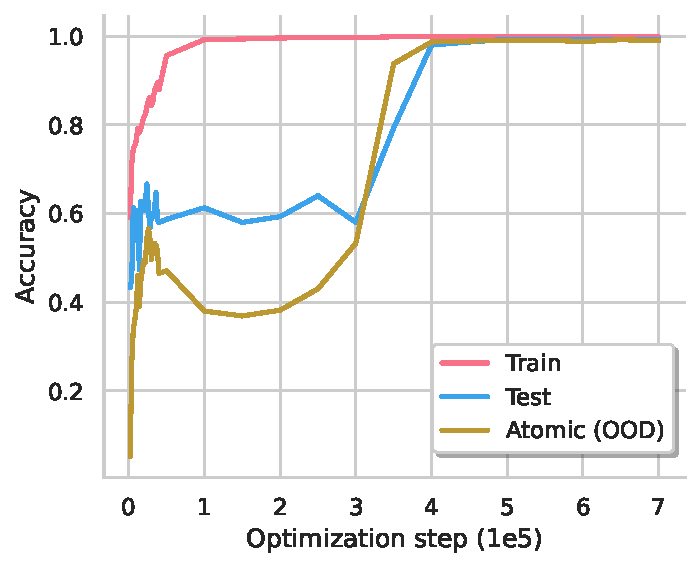
\includegraphics[width=0.6\textwidth]{fig/grokking_hr.pdf}
\caption{Accuracy on the train and test split, and also the accuracy of inferring the attribute values of the query entities (\textbf{Atomic (OOD)}) for the complex reasoning task in \S\ref{sec:hard_reasoning}.}
\label{fig:hr}
\end{figure}
